\section{Relacijski model podataka}

Nakon uspješno provedene analize podataka, sljedeći korak u razvoju skladišta podataka predstavlja kreiranje relacijskog modela koji će osigurati strukturirano i normalizirano čuvanje podataka. Relacijski model omogućuje organizaciju podataka u tablice povezane preko stranih ključeva, što omogućava efikasno dohvaćanje i manipulaciju podataka \cite{Elmasri2017}.

\subsection{Analiza entiteta i atributa}

Temeljito razumijevanje strukture podataka o automobilima omogućilo je identifikaciju ključnih entiteta koji će činiti okosnicu relacijskog modela. Kroz analizu originalnog skupa podataka identificirani su sljedeći glavni entiteti:

\textbf{Osnovni entiteti:}
\begin{itemize}
    \item \textbf{Automobil} - središnji entitet koji sadrži osnovne karakteristike vozila
    \item \textbf{Proizvođač} - entitet koji predstavlja tvrtke koje proizvode automobile
    \item \textbf{Model} - specifični model automobila određenog proizvođača
    \item \textbf{Zemlja} - zemlja podrijetla proizvođača
    \item \textbf{Regija} - geografska regija kojoj pripada zemlja
\end{itemize}

\textbf{Klasifikacijski entiteti:}
\begin{itemize}
    \item \textbf{Tip mjenjača} - klasifikacija prema vrsti transmisije
    \item \textbf{Tip goriva} - kategorije goriva koje automobil koristi
    \item \textbf{Desetljeće} - vremenski period proizvodnje
    \item \textbf{Kategorija starosti} - klasifikacija prema godinama starosti
    \item \textbf{Kategorija kilometraže} - klasifikacija prema prijeđenim kilometrima
    \item \textbf{Klasa veličine motora} - kategorije prema volumenu motora
\end{itemize}

Ova kategorizacija omogućuje stvaranje normaliziranog modela koji minimizira redundanciju podataka i omogućuje efikasne upite.

\subsection{Konceptualni model podataka}

Konceptualni model predstavlja visokorazinsku apstrakciju poslovnih zahtjeva bez ulaska u tehnička ograničenja. Za potrebe ovog projekta definiran je model koji odražava prirodne veze između entiteta u domeni trgovine automobilima.

Ključne veze u modelu uključuju:
\begin{itemize}
    \item Svaki automobil pripada određenom modelu (1:N)
    \item Svaki model proizvodi točno jedan proizvođač (1:N)
    \item Svaki proizvođač dolazi iz jedne zemlje (1:N)
    \item Svaka zemlja pripada jednoj regiji (1:N)
    \item Automobil ima jednu kategoriju za svaki klasifikacijski atribut (1:N)
\end{itemize}

\begin{figure}[H]
    \centering
    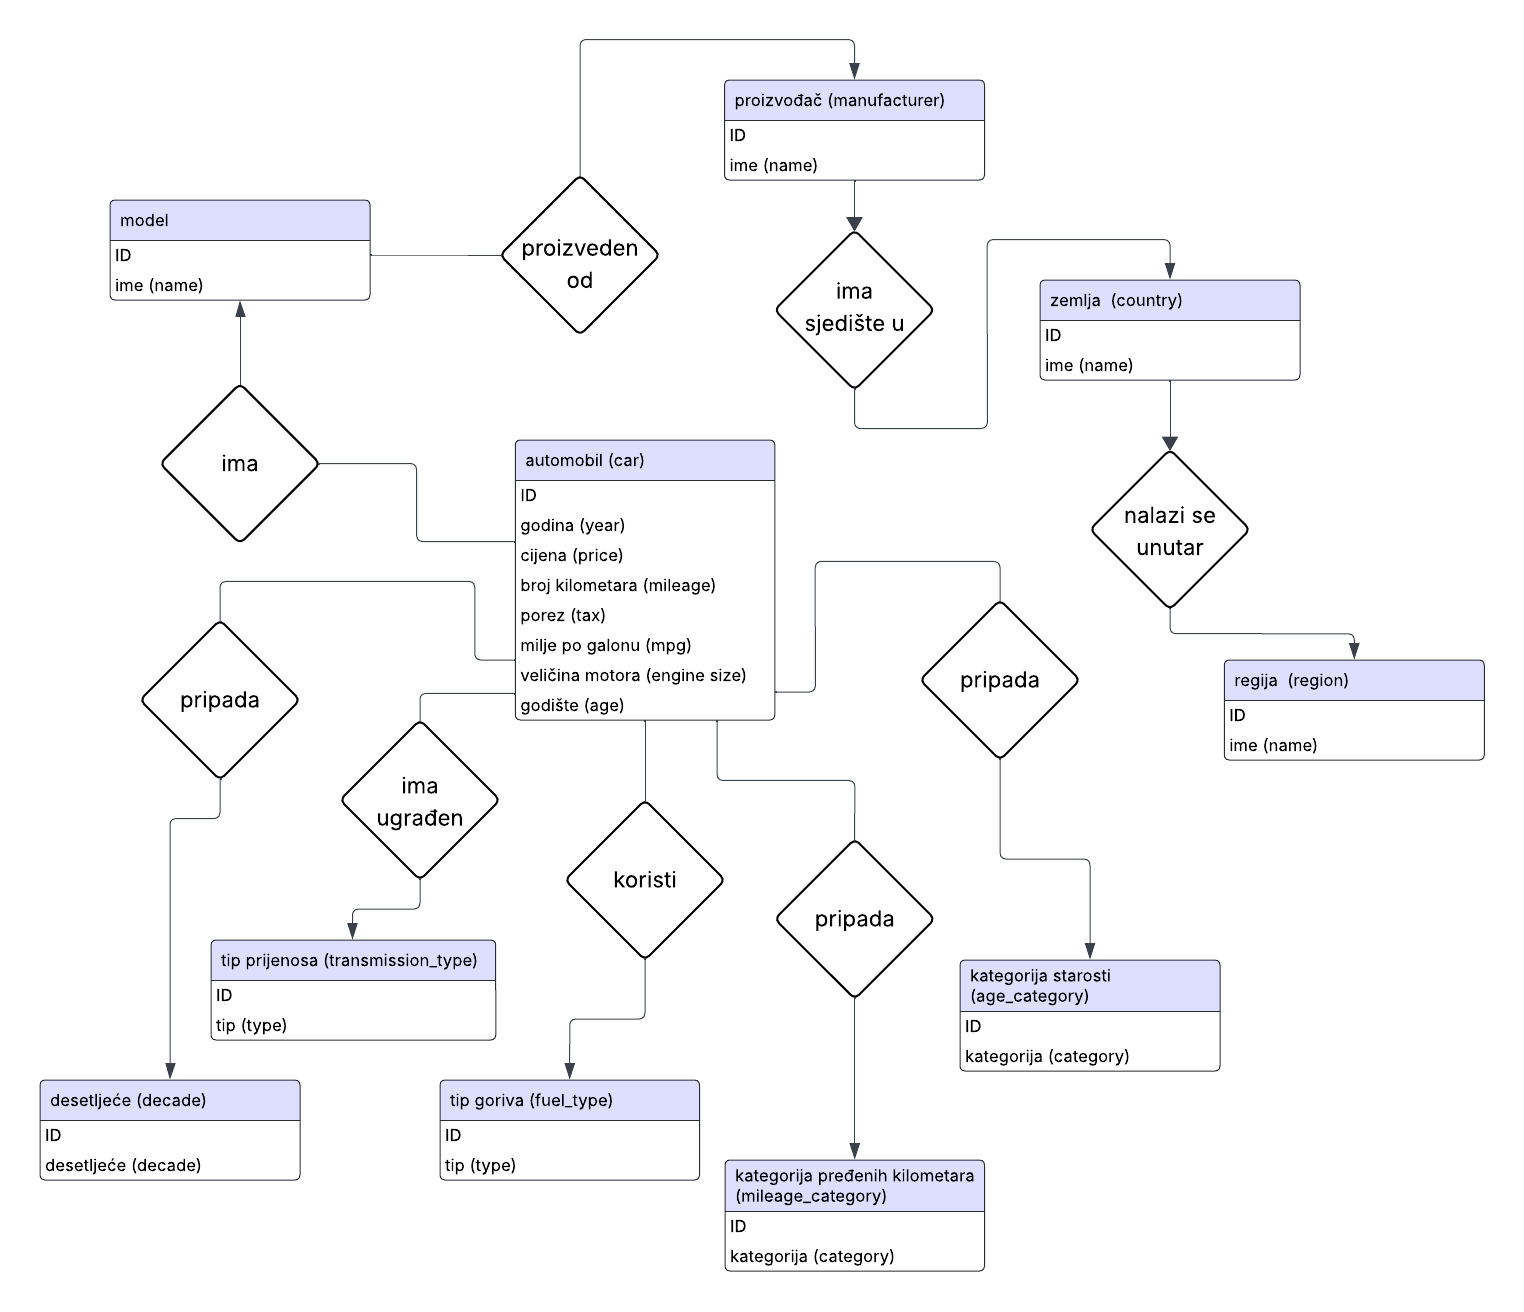
\includegraphics[width=0.9\textwidth]{slike/relational_model/er-dijagram.png}
    \caption{Konceptualni Entity-Relationship dijagram}
    \label{fig:er-dijagram}
\end{figure}


ER dijagram prikazuje kompletan konceptualni model s entitetima, atributima i vezama između njih. Dijagram je kreiran koristeći standardnu notaciju koja jasno označava kardinalnosti i ograničenja. Na dijagramu je jasno vidljiva hijerarhijska struktura od regije do modela automobila, kao i klasifikacijski entiteti koji omogućuju analitičko izvještavanje. Svaki entitet sadrži primarni ključ i relevantne atribute koji podržavaju analitičke zahtjeve.

\subsection{Implementacija relacijskog modela}

Logički model podataka implementiran je koristeći MySQL bazu podataka, pri čemu je osobita pozornost posvećena normalnim formama i referencijalnim ograničenjima. Model slijedi treću normalnu formu (3NF) što osigurava minimizaciju redundancije podataka.

\begin{figure}[H]
    \centering
    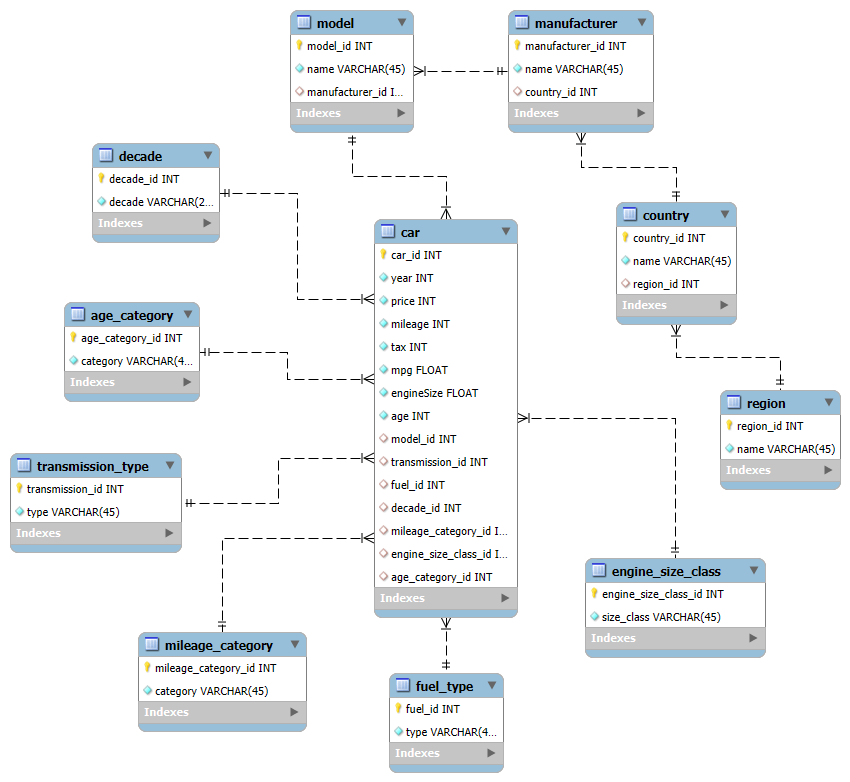
\includegraphics[width=1.0\textwidth]{slike/relational_model/relacijski-model.png}
    \caption{Implementirani relacijski model u MySQL bazi podataka}
    \label{fig:relacijski-model}
\end{figure}

Implementacija uključuje:
\begin{itemize}
    \item \textbf{Referencijalnu cjelovitost} - svi strani ključevi osiguravaju postojanje povezanih zapisa
    \item \textbf{Jedinstvene ograničenja} - sprječavanje dupliciranja entiteta
    \item \textbf{NOT NULL ograničenja} - osiguravanje kompletnosti kritičnih atributa
    \item \textbf{Auto-increment primarni ključevi} - efikasno upravljanje identifikatorima
\end{itemize}

\subsection{Automatizacija kreiranja i popunjavanja baze}

Za potrebe reproducibilnosti i održivosti projekta razvijene su Python skripte koje automatiziraju proces kreiranja i popunjavanja baze podataka. Glavna skripta koristi SQLAlchemy ORM za definiranje sheme baze.

\begin{lstlisting}[language=Python, caption={Definiranje ORM modela za glavni entitet automobila}]
class Car(Base):
    __tablename__ = 'car'
    car_id = Column(Integer, primary_key=True, autoincrement=True)
    year = Column(Integer, nullable=False)
    price = Column(Integer, nullable=False)
    mileage = Column(Integer, nullable=False)
    tax = Column(Integer, nullable=False)
    mpg = Column(Float, nullable=False)
    engineSize = Column(Float, nullable=False)
    age = Column(Integer, nullable=False)
    
    # Strani kljucevi
    model_id = Column(Integer, ForeignKey('model.model_id'))
    transmission_id = Column(Integer, ForeignKey('transmission_type.transmission_id'))
    fuel_id = Column(Integer, ForeignKey('fuel_type.fuel_id'))
    # ... ostali strani kljucevi
\end{lstlisting}

Proces popunjavanja baze provodi se u kontroliranim fazama:
\begin{enumerate}
    \item \textbf{Kreiranje osnovnih entiteta} - regije, zemlje, proizvođači
    \item \textbf{Kreiranje klasifikacijskih tabela} - tipovi goriva, mjenjača, kategorije
    \item \textbf{Kreiranje modela} - povezivanje s proizvođačima
    \item \textbf{Umetanje automobila} - povezivanje sa svim referentnim entitetima
\end{enumerate}

\subsection{Validacija podataka i testiranje}

Za osiguravanje ispravnosti procesa migracije podataka u zasebnoj skripti implementiran je sveobuhvatan sustav testiranja koji uspoređuje originalne CSV podatke s podacima u bazi.

\begin{lstlisting}[language=Python, caption={SQL upit za rekonstrukciju originalnih podataka}]
query = """
SELECT mfg.name as 'manufacturer', mdl.name as 'model'
, c.year, c.price, c.mileage, c.tax, c.mpg, c.engineSize
, t.type as 'transmission', f.type as 'fuelType'
, d.decade, cnt.name as 'country', r.name as 'region'
, mc.category as 'mileageCategory'
, esc.size_class as 'engineSizeClass'
, c.age, ac.category as 'ageCategory'
FROM car c
JOIN model mdl ON c.model_id = mdl.model_id
JOIN manufacturer mfg ON mdl.manufacturer_id = mfg.manufacturer_id
-- ... ostali JOIN-ovi
ORDER BY c.car_id ASC
"""
\end{lstlisting}

Test provjerava:
\begin{itemize}
    \item \textbf{Integritet strukture} - postojanje svih stupaca u bazi
    \item \textbf{Kompletnost podataka} - broj zapisa u bazi odgovara CSV datoteci
    \item \textbf{Ispravnost sadržaja} - vrijednosti u bazi identične su originalnim podacima
    \item \textbf{Referencijalnu konzistentnost} - svi strani ključevi ispravno povezani
\end{itemize}
